In order to study the effect of communication networks around cryptocoins on
price variations, we collected all the posts from the most popular cryptocurrency
online community, \url{https://bitcointalk.org}.  Our data consists of all the posts that were
made between January 2010 and July 2015 on the most active crypto-related forums:
\begin{enumerate}[topsep=0pt,itemsep=-0.5ex,partopsep=1ex,parsep=1ex]
  \item \textbf{Bitcoin Discussion:} This is the oldest forum on the website which mainly focuses
    on issues related only to Bitcoin. Interestingly, Satoshi Nakamoto, the alleged
    creator of Bitcoin made the first post on this forum in January 2010 and
    was active until January 2011. The presence of Satoshi in the data set enables us
    to study the position of various actors in the online community relative to Satoshi
    and its relation with the success or failure of cryptocoins they advocate or reject.
    %JULIAN: Why is people's relationship to Satoshi likely to be interesting or important?
  \item \textbf{Altcoin Discussion:} This is the most active forum in the community
    with more than 730,000 posts as of July 2015, dating back to June 2011.
    The discussions in this forum mainly evolve around alternative currencies
    other than Bitcoin. Users often discuss the merits or flaws of various
    altcoins or simply exchange technical information.
  \item \textbf{Announcement (Altcoin):} Community announcements such as development of 
    exchange clients or addition of new features are made here. This is an important forum
    in our study as the creation of new altcoins are announced here. Whenever a new
    altcoin is announced to the community, the announcement is tagged with string ANN.
    This enables us to detect announcements of new coins into the market and identify
    the users who introduced them for the first time.
  \item \textbf{Mining (Altcoin):} Technical issues pertaining to mining (i.e.~validating transactions)
    altcoins are discussed here.
  \item \textbf{Marketplace (Altcoin):} This forum contains the discussions on a wide-range of 
    market-related issues, such as price or volume trends, possible pump-and-dump schemes
    and exchange tips.
\end{enumerate}

Each forum consists of many subjects or threads initiated by different users.
Each thread contains several posts or replies, with an average of 10 posts per
thread.  The reply structure within each thread constitutes the basis of our
forum network, discussed below.  Each post has several fields which contain
valuable information in our context.
\begin{enumerate}[topsep=0pt,itemsep=-0.5ex,partopsep=1ex,parsep=1ex]
  \item \textbf{Subject:} Usually, the initiator of the thread chooses subject and all the
    following posts inherit the same subject.
  \item \textbf{Content:} The actual text of the post.
  \item \textbf{Position in the thread}: The later posts in the thread might not be as important
    as earlier posts and could be about issues other than the original topic of the thread.
  \item \textbf{Author}
  \item \textbf{Date}
\end{enumerate}
The community had only 10,000 unique users until early 2013, however it grew considerably faster after 2013 and reached about 70,000 by early 2015.
Nevertheless, there are only around 10,000 active users within any 30 day period on average.
Figure \ref{aurora_thread} shows an example of the first post in a thread which introduced Aurora coin for the first time in the Announcement forum.

\begin{figure}
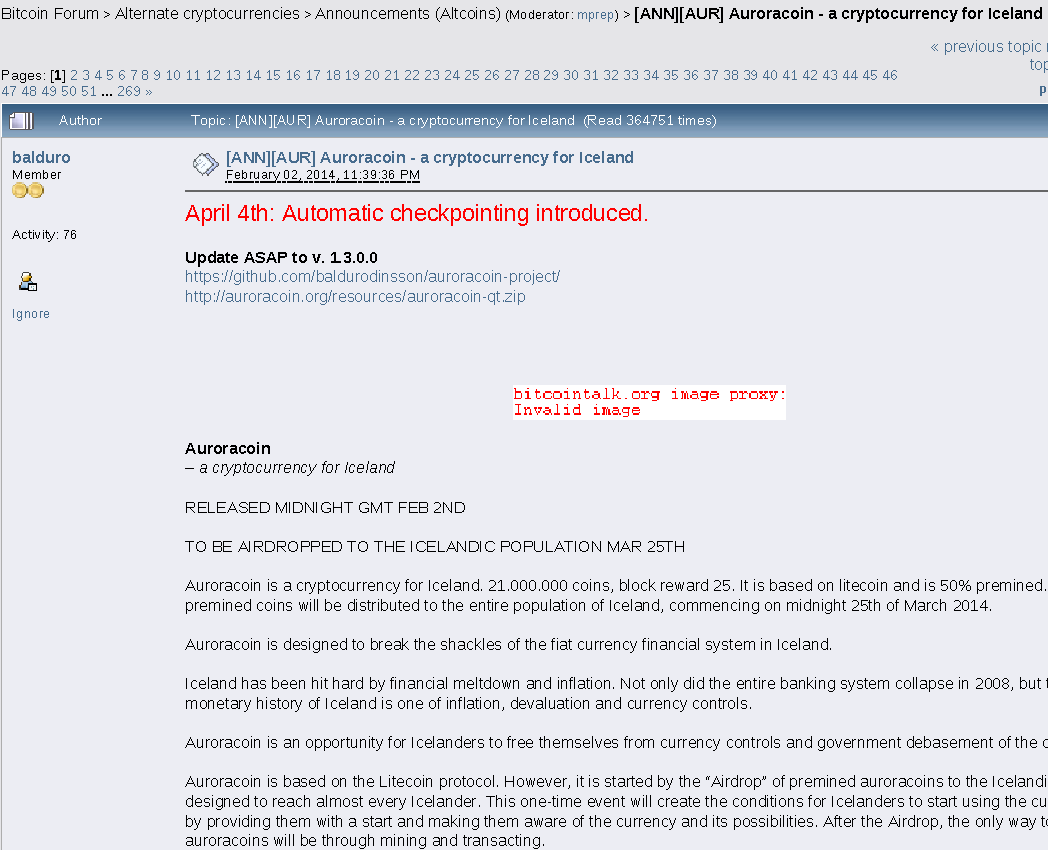
\includegraphics[width=0.99\columnwidth]{aurora_thread_cut.pdf}
\caption{The first post of a thread announcing the release of Auroracoin for the first time in \url{https://bitcointalk.org} \textcolor{red}{remove?}}
\label{aurora_thread}
\end{figure}

%JULIAN: Being crass, just showing a quick figure with an example of a discussion wouldn't hurt. I have no idea what people discuss on forums like this, so a figure whose purpose is to convince me that there's meaningful signal here could be helpful
